\section{Anonymization}

Anonymization of personal data refers to the process of removing personally identifiable information (PII) from data sets so that the individuals represented in the data cannot be identified. This is accomplished by either completely removing or replacing identifiable data with generic values. The purpose of anonymization is to protect the privacy of individuals while still allowing the data to be used for legitimate purposes. \\
Most of the recent implementations of anonymization works by masking the personal information of a person, such as names and surnames, telephone numbers, addresses, credic card numbers and so on. \\
One of the most famous library for anonymization is Presidio, developed by Microsoft. Presidio exploits pattern recognition with regex and Named Entity Recognition to find all the personal information of mask them. \\
The main disadvantage of such techniques is that often the personal subject can be identified through the so-called quasi-identifiers, that more often than not are not masked.
\\Here reported some examples that are not masked by Presidio:\\ \\
Original sentence
\begin{adjustwidth}{1cm}{}
    The new intern at my office, the one with red hair, caught covid last week 
\end{adjustwidth}
Sentence redacted by Presidio
\begin{adjustwidth}{1cm}{}
    The new intern at my office, the one with red hair, caught covid \textless DATE\_TIME \textgreater
\end{adjustwidth}
Original sentence
\begin{adjustwidth}{1cm}{}
    The boss of the HR department of has made some weird comments about how I dress
\end{adjustwidth}
Sentence redacted by Presidio
\begin{adjustwidth}{1cm}{}
    The boss of the HR department of has made some weird comments about how I dress 
\end{adjustwidth}
Our new approach exploits a Sequence to Sequence model called T5
T5 is a model released by Google in 2019, it is a standard encoder-decoder transformer which, unlike BERT, always returns strings as outputs. This is why it is called a sequence to sequence model. \\
T5 is a unified model that can be applied for many downstream tasks, such as sentiment analysis, sentence completation, question answering\dots\\
In T5 architecture there are \textit{adapted layers} after each feed forward layer, whose scope is to diminish the number of parameters updates for each fine-tuned model. In fact, \textit{adapted layers} are dense-ReLU-dense blocks that are designed so that their input dimensionality and output dimensionality are equal. This let us to insert them into the Transformer architecture without other changes. When fine-tuning for each different task, only the \textit{adapted layers} and the normalization layers will be updated. This results in a considerable reduction of parameters updates.\\
We followed a few-shot learning approach with T5. Rather than relying on a large amount of training data to allow a pre-trained model to adjust to a given task accurately, few-shot learning employs the use of a few examples to direct the training of a machine learning model with very minimal data. \\
For each category of tickets, we wrote 10 examples of "anonymized" tickets , where we removed all personal information and information that could retrace to the original writer, maintaning only information that could be useful for analysis purposes.
Here a couple of examples:\\ \\
Original sentence:
\begin{adjustwidth}{1cm}{}
    Dear Sir/Madame, I cannot stand anymore this discrimination and prejudice against French people at work
\end{adjustwidth}
Anonymization used for few-shot learning:
\begin{adjustwidth}{1cm}{}
    The employee is filling a complaint for discrimination based on nationality 
\end{adjustwidth}
Original sentence:
\begin{adjustwidth}{1cm}{}
    Hello, my name is Zacaredas Pinilla and I work at Laguna-Franco Spain. I am having trouble finding an accommodation in the Algeciras area so if you could help me with this matter it would be greatly appreciated
\end{adjustwidth}
Anonymization used for few-shot learning:
\begin{adjustwidth}{1cm}{}
    The employee is asking for help finding an accommodation
\end{adjustwidth}
\begin{figure}[h] 
    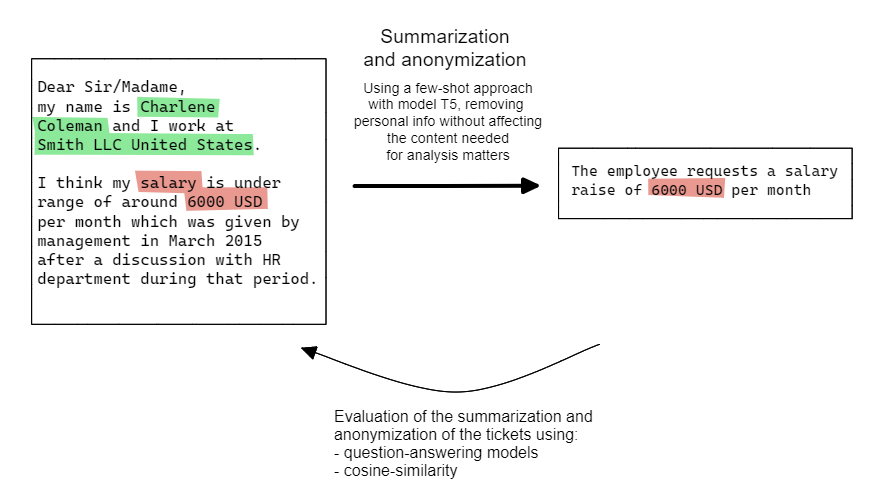
\includegraphics[width=\textwidth]{images/ticket_anonymization_schema.png}
    \caption{Schema of Ticket Anonymization}
    \label{fig:schema_ticket_anonymization}
\end{figure}    
To evaluate the goodness of an anonymization and how much of the information has remained after the anonymization we have used three different methods:
\begin{itemize}
    \item \textbf{QAGS}: Questions Answering and Generation for summarization
    \item \textbf{SUMMAQA}: Unsupervised metric for reinforced summarization model 
    \item \textbf{Cosine Similarity}
\end{itemize}  
These models were originally created to evaluate the goodness of a summarizatoin, we have adapted them to be used for evaluating our anonymization. \\
The first two methods follow the same philosophy: they generate questions to ask both the original version and the anonymized version of the tickets, looking if the answers are coherent. We call them Questions and Answers models.

\subsection*{QAGS}
\subsection*{SUMMAQA}
\subsection*{Cosine Similarity}

\begin{figure}[h] 
    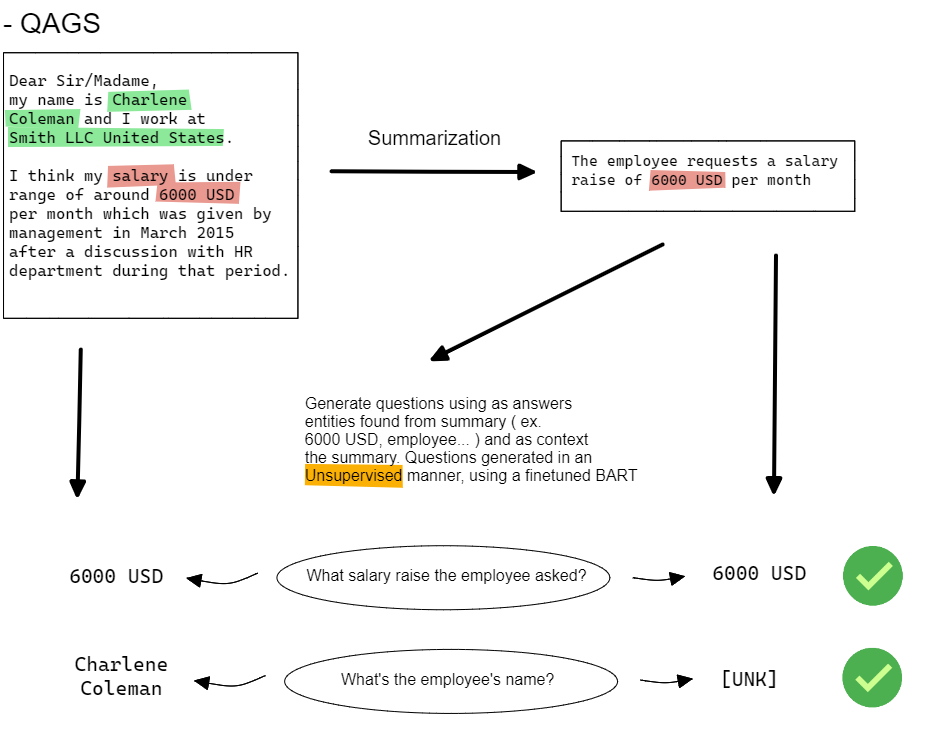
\includegraphics[width=\textwidth]{images/qa_models_qags.png}
    \caption{Schema of QAGS}
    \label{fig:schema_qags}
\end{figure}    

\begin{figure}[h] 
    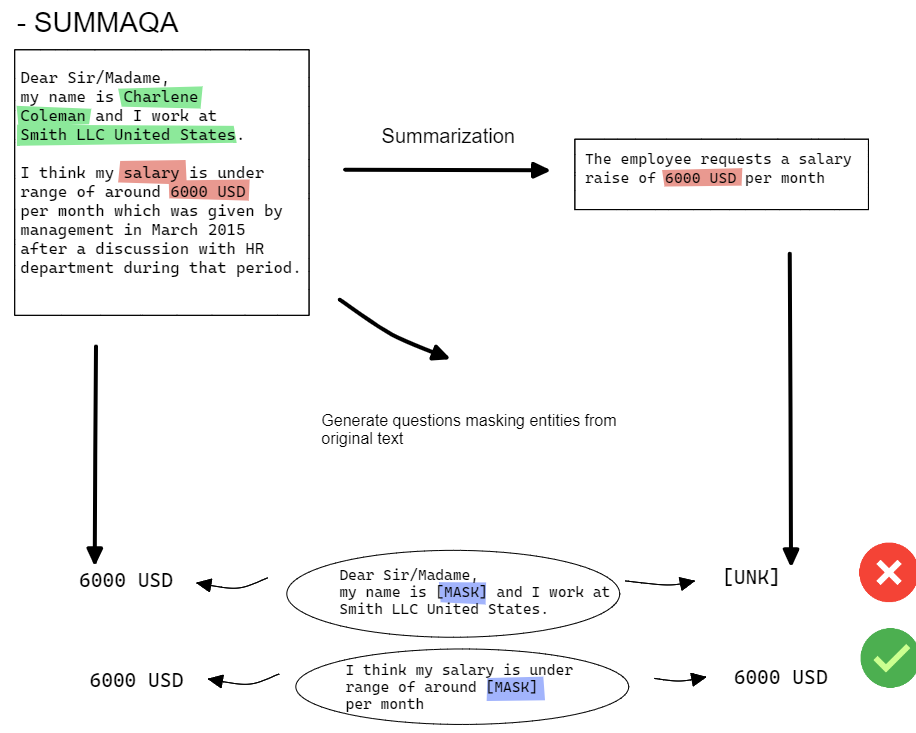
\includegraphics[width=\textwidth]{images/qa_models_summaqa.png}
    \caption{Schema of SUMMAQA}
    \label{fig:schema_summa_qa}
\end{figure}    

\begin{figure}[h] 
    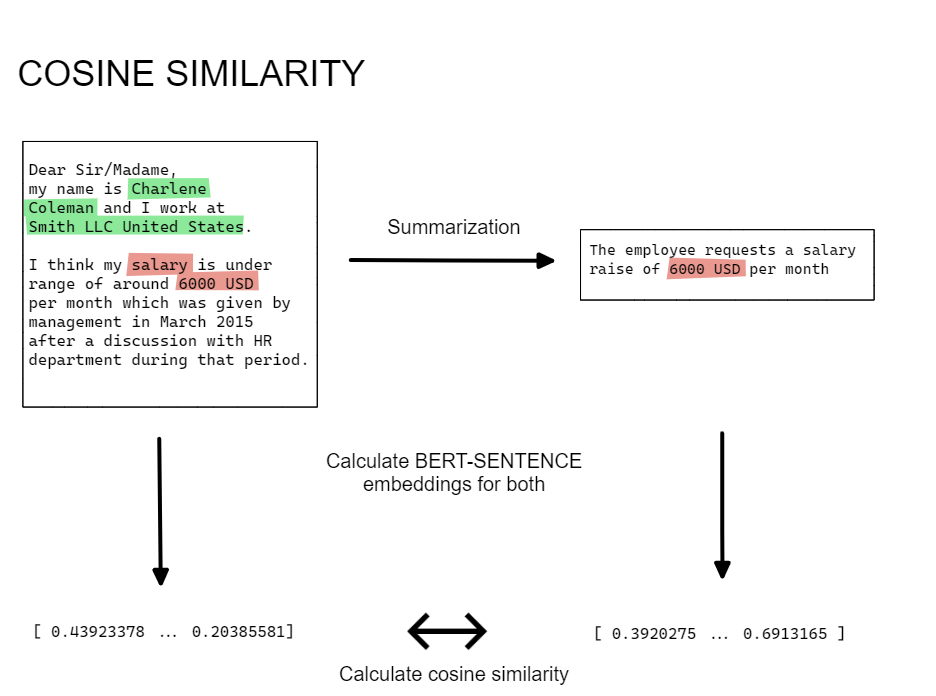
\includegraphics[width=\textwidth]{images/cosine_similarity.png}
    \caption{Schema of Cosine Similarity for }
    \label{fig:schema_cosine_similarity}
\end{figure}    




